\documentclass{article}
\usepackage{aaai}
\usepackage{fixbib}
\usepackage{amsmath}
\usepackage{graphicx}
\usepackage{times}
\usepackage{helvet}
\usepackage{courier}
\usepackage{graphicx}
\usepackage{multirow}
\usepackage{verbatim}
\usepackage{url}
\usepackage[utf8]{inputenc}
\DeclareUnicodeCharacter{FB01}{fi}
\graphicspath{ {images/} }
\frenchspacing
\setlength{\pdfpagewidth}{8.5in}
\setlength{\pdfpageheight}{11in}


\title{
	CS4246 AI Planning and Decision Making - Project 2 \\
	Planning and Decision Making Automation on Depression
}
\author{
	{\bf Team 01} \\
	Antoine Charles Vincent Garcia - A0159072A\\
	Chan Jun Wei - A0112084U\\
	Chen Tze Cheng - A0112092W\\
	Eric Ewe Yow Choong - A0112204E\\
	Han Liang Wee, Eric - A0065517A\\
	Ho Wei Li - A0094679H\\
}

\begin{document}
 	\maketitle

	\begin{abstract}
	\begin{quote}
	Depression is a debiliatating mental illness that has good prognosis given early detection and treatment. 
	However, detection is difficult with the various factors that raise the entry barriers and decrease the accuracy of a diagnostic test. Research have shown that accurate predictions of emotions can be made with Gaussian Process models. 
	This study explores the novel use Gaussian Process in predicting depression severity using acoustic measures of voice.
	Our work has succesfully shown that Gaussian Process Dot Product trained using MFCC feature set is a good model for depression prediction and can predict PHQ-8 better than other state-of-the-art models at RMSE of 6.34.\\
	\end{quote}
	\end{abstract}
	
	\section{Introduction}
	Depression has a severe, and at times long-term, negative impact on an individual's quality of life. 
	Major depression is 3rd leading cause of disability worldwide with 65 million life years spent living with the disability or lost due to early death \cite{who2004}.
	Depression's annual toll on U.S businesses amounts to about \$80 billion in medical expenditures, lost productivity and suicide. 
	Among the costs, close to \$10 billion accrued in lost workdays each year and more than \$33 billion in other costs accrue from decreased productivity due to symptoms that sap energy, affect work habits, cause problems with concentration, memory, and decision-making \cite{tjcp2015}. \\

	Left unchecked, depression increases risk for morbidity, suicide, decreased cognitive and social functioning, self-neglect, and early death \cite{arcp2009}. 
	Death from suicide is one of the top 10 causes of death, above the death rate for chronic liver disease, Alzheimer's, homicide, arteriosclerosis or hypertension \cite{nvsr2016}. \\

	Despite the severe consequences, depression is one of the most treatable mental illnesses but it is also one of the most under-diagnosed globally. 
	In general health-care, 48.4\% of patients suffering from depression go unrecognized \cite{jama2003}.

	\subsection{Motivation and Objective}
	The Personal Health Questionaire depression scale (PHQ-8) is a self-administered, 8-question diagnostic test for depressive disorders that has proven to be an effective severity measure for depression in large clinical studies \cite{jad2008}. 
	Nevertheless, one of the biggest obstacles to successful diagnosis of depression is the unwillingness of patients to admit their predisposition to depression by seeking help.\\

	People often subscribe to the social stigma that being depressed reflects a weakness in their character, a permanent defect in their personality. 
	This stigma manifests itself particularly in a phenomenon known as social distancing whereby people with mental issues are more isolated from others \cite{tpcrp2011}.  
	People suffering from depression hence tend to be ashamed of their condition and are generally convinced that denying and hiding it from others gives them a better shot at integrating with society and living a normal life \cite{bmb2001}.
	Even if they do seek help, the accuracy of the PHQ-8 or just questionaires and surveys in general are often adversely affected by the Hawthorne Effect, 
	a type of reactivity in which individuals modify or improve an aspect of their behavior in response to their awareness of being observed. \cite{jce2014}.\\

	In the past decade, there have been research successfully correlating emotion with voice production and speech acoustics \cite{uwa2001}. 
	Corollary to that, active research of late into the use of voice acoustics as predictors of clinical depression scores has seen success, proving that it is an effective indicator of depression severity \cite{jov2016}.\\

	In this paper, we investigate the applicability and feasibility of Gaussian Process (GP) models in predicting clinical ratings of depression severity on the PHQ-8 scale with acoustic measures of voice from a sample of patients and compare their performance with current state-of-the-art machine learning models. 
	Some of our preliminary studies have shown that despite consensus among the scientific community that Support Vector Machine (SVM) models have a 
	very high predictive accuracy specifically in speech emotion recognition \cite{Chavhan2010}, GP models have been proven to consistently outperform SVM models on the task of music emotion recognition \cite{MARKOV2013}. 
	Nevertheless, there are no studies on the use of GP in predicting depression severity. 
	The findings of this paper will hopefully open up new frontiers and fuel further research interest on this topic. 
	
	\subsection{Important Requirements}
	...
	
	\section{Modelling and Approach}
	Leveraging on the success of the modelling of depression prediction of PHQ-8 scores in project 1, we extend and apply the work done to solve the aforementioned problem of under-staffing. 
	Our solution is to implement pre-screening and automate the process of the deciding if the person needs an appointment or otherwise. 
	Moreover, our process allows prioritizing of patient's appointments by their PHQ-8 score. 
	Henceforth, we would need to use 2 GPs: Gaussian Process Classifier (GPC) and the Gaussian Process Regressor (GPR). 
	In this section, we will firstly describe the process that we are proposing and we will go into detail on each component of the process.

	\subsection{Automation Flow} \label{af}
	\begin{figure}[h]
 		\begin{center}
		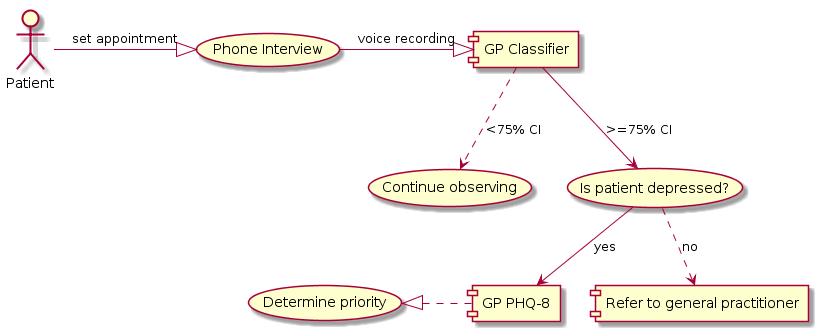
\includegraphics[width=0.48\textwidth]{automation} 
  		\end{center}
  		\caption{Automation Flow}
  		\label{auto_flow} 
 	\end{figure}
 	\begin{comment}
	@startuml
		Patient -right-|>(Phone Interview) : seek treatment
		(Phone Interview) -right-|> [GPC] : voice recording
		(Set appointment) --> [GPC] : repeat process after a time t
		[GPC] --> (Schedule appointment) : < p
		[GPC] --> (Is patient depressed?) : >= p
		(Is patient depressed?) ..> (Schedule appointment ) : yes
		(Is patient depressed?) ..> (No appointment needed) : no
	@enduml
 	\end{comment}

	As shown in Figure \ref{auto_flow}, the model is the steps of an average user who is seeking for medical attention in the early stages of depression.
	Prior to medical treatment, the patient is required to call up a psychiatrist to arrange an appointment time and date. 
	At that time, a short phone interview consisting of a fixed number of unbiased questions is conducted.
	The objective of the interview is to record the patient's voice pattern.
	The recordings will the serve as an input for the first GP, which is a classifier that will output both the confidence interval and a binary state to whether the patient is suffering from depression or not.
	This leads to two scenarios depending on the \emph{p}, which is the probability estimate:
	
	\begin{enumerate}
		\item {\textgreater= \emph{p}} \\
		The patient's affliction diagnosable.
		However, this is also dependent on the binary state i.e. whether the patient is depressed or not depressed. 
		A depressed patient will be given further attention by the psychiatrist by scheduling an appointment whereas a non-depressed patient would be not be given attention by the psychiatrist.
		\item {\textless \emph{p}} \\
		The patient's affliction is uncertain. 
		In this case, the patient can still schedule an appointment and is placed under continuous scrutiny until he/she can be diagnosed as depressed or vice versa.
		This outcome is not unusual as depression is disorder can be recurrent and often in episodes \cite{bp6152013}, a prediction generated over a time span therefore produces more accurate results.\\
	\end{enumerate}
	
	\begin{figure}[h]
 		\begin{center}
		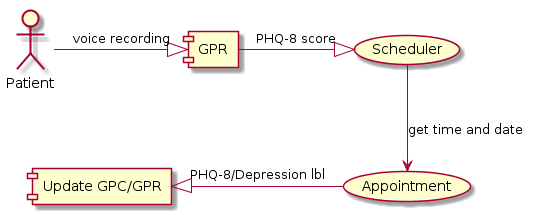
\includegraphics[width=0.48\textwidth]{appointment} 
  		\end{center}
  		\caption{Flow for Scheduling an Appointment}
  		\label{sch_app} 
 	\end{figure}
 	\begin{comment}
	@startuml			
		[Voice recording] -right-|> [GPR] : input
		[GPR] -right-|> (PHQ-8 Score) : outputs
		(PHQ-8 Score) -right-|> [Scheduler] : feed to
		[Scheduler] --> (Appointment) : get time and date
		(Appointment) -left-|> (PHQ-8/Depression LBL)
		(PHQ-8/Depression LBL) -left-|> [Update GPC/GPR] : use to
	@enduml
 	\end{comment}

	Continuing from Figure \ref{sch_app} after the psychiatrist has agreed for an appointment, the voice of the patient will then be used as an input for the GPR which models the PHQ-8. 
	This is to determine the scale of depression that the patient is suffering from which also helps the psychiatrist to select an appropriate appointment date. 		
	Similar the to the triage procedure in emergency services, a patient with a higher PHQ-8 value will be placed on the higher end of the priority list and vice versa.
	The patient's LBL and PHQ-8 scores will be observed over time during scheduled sessions to identify the patient's improvement in his/her emotional state.
	All the data gathered, will then be fed into the GPC and GPR until there is an improvement in the results.
	Undiagnosable patients undergo the same process until he/she can be given a proper classification of whether he/she is depressed or not.
	From here on, he will also undergo the process in \ref{sch_app} or is refuse an appointment if found that he/she is not depressed.

	\subsection{Insights to our model}
	\subsubsection{Gaussian Processes :}
	In our modelling, we used 2 gaussian processes(GP) for regression and classification tasks respectively. 
	The GP models that we use here are modelled similarly to the modelling done in project 1. 
	GPR predicts the (Personal Health Questionaire depression scale)PHQ-8 score, while GP classifier(GPC) predicts whether the person is depressed or not. 
	Similar to project 1, we trained GPR and GPC with data obtained from Audio/Visual Emotion Challenge and Workshop (AVEC 2016) \cite{avec2016}, with PHQ-8 and depression labels respectively. 
	We applied the same audio signal processing techniques to the audio files as per project 1. 
	We only used the Mel Frequency Cepstral Coefficients (MFCC) feature subset as we have seen the good theorical and experimental results the feature subset had produced. 
	Most importantly, we make the same two assumptions so that the GP model planning and decision making is suitable for depression prediction:
	\begin{enumerate}
		\item Depression prediction is an event-based recognition which provides a single depression estimate over a certain amount of time. \cite{Valstar2016}
		\item The speech signals extracted from different people suffering from depression should share some similarities and thus admissible for prediction with the Gaussian Process models\cite{Cummins2015}.
	\end{enumerate}
	Since the GP models recieve new data incrementally, we cannot use an offline GP as per project 1. 
	Hence, we would need to tweak the GP to fit this problem. Since it is not possible for us to obtain a comprehensive dataset of all people coming to the clinic, we would then need a GP that learn dynamically, adapting to new data as it becomes avaliable. 
	Online machine learning is a method that allows the data to be updated when it becomes available. 
	We have noted that there are online variants of GP, namely: XXYY, XXYYX and XXHS. It is with this reasoning that we chose this particular online variant of GP. 
	
	\subsubsection{Phone Interview :}
	We note that regardless of the questions asked or the circumstance, a depressed person will still exhibit signs of depression in his speech\cite{jad2008}. 
	Hence, the questions asked are irrelevant. The questions will be presented in the proof of concept section.

	\subsubsection{Decision making :}
	The greatest advantage of using GP over other machine learning algorithms is that it provides us with a probability estimate representing confidence of the prediction. 
	With that probability, we can decide if the predicted label can be relied on or that it cannot be trusted and needs to learn this data point. In our model, we exploit this property, unique to GPs. 
	After the interview, GPC will predict the depression label with a confidence $p_c$ on the audio recording. 
	As mentioned in the modelling, we define a particular probability $\rho_c$. If GPC predicts with $p_c>\rho_c$, then we can trust the predicted label and continue to decide appropriately based on the label. 
	We determine the probability $\rho_c$ experimentally by observing the prediction quality of the labels in the training data, a summary is given in table \ref{tab:rho}.
	
 	\begin{table}[h]
 		\begin{center}
  			\begin{tabular}{ | r | c | c | }
    			\hline
			 	 \bfseries $p_c$($\%$)	& \bfseries Depression 	& \bfseries No Depression \\ \hline
				 $[0,10)$		& - 			& - 			 \\ \hline
				 $[10,20)$		& $100\%(1/1)$ 		& -		 \\ \hline
				 $[20,30)$		& $100\%(4/4)$ 		& - 	 \\ \hline
				 $[30,40)$		& 95 			& $100\%(1/1)$ 			 \\ \hline
				 $[40,50)$		& 6.326 		& 7.548		 \\ \hline
				 $[50,60)$		& 5.597 		& 6.690 	 \\ \hline 
				 $[60,70)$		& $100\%(1/1)$ 			& 31 			 \\ \hline
				 $[70,80)$		& - 		& $100\%(1/1)$		 \\ \hline
				 $[80,90)$		& - 		& $100\%(4/4)$ 	 \\ \hline 
				 $[90,100]$		& - 			& - 			 \\ \hline
				 -		& 95 			& 31 			 \\ \hline
			 \end{tabular}
		\end{center}
 	\caption{Relationship between probability and accuraccy... Fix table later}
 	\label{tab:rho}
 	\end{table}

	\subsubsection{Scheduling :}
	For the cases when the person needs to be scheduled for an appointment with the psycharist, we can use GPR to determine the predicted PHQ-8 scores. 
	With the predicted scores, we can piroritise certain higher risk individuals over the rest. 
	Since the depression clinic is understaffed and struggling to keep up with number of patients, it is wise to piroritize the individuals who are predicted with higher PHQ-8 scores, which indicates that they are likely to be more depressed. 
	Hence, we optimize the scheduling piroritizing people with higher predicted PHQ-8 scores.

	\subsection{Qualitative Advantages}
	The greatest advantage of using a GP is that it provides us with a probability estimate along with the predicted label. 
	We rely on the probability to determine the reliability of the predicted label. 
	As we are dealing with human beings, we would want to rely on the predicted label only if it is reliable. 
	Additionally, we have read in medical literature regarding the dire consequences of misdiagnosis and/or inappropriate treatment\cite{nasrallah2015consequences,bowden2001strategies,dunner2003clinical} in the area of depression. 
	With the probability, we can be confident of the decisions that we make, that can potentially affect a person. 
	Assume that we have a predicted label that can be trusted, then with the label, i.e. true for depressed and false for not depressed, we can decide if the person needs to come to the clinic for an appointment. 
	Hence, reducing the number of appointments that are made, easing the workload of the staff in the clinic. \\
	
	In addition to reducing the workload of the staff, the GP models can potentially improve as more patients go through the pre-screening process.
	It can be the case that the GP is not confident of its prediction, then we should not trust the label that the GP had predicted. 
	Then, we would need to determine by the means of a physical examiniation if the person in question is depressed or not and administer the appropriate treatment. 
	Through the appointment with the psychiatrist, he can determine if the patient is depressed or not. 
	With the ground truth, we can now train the GPs with the new data point. We are also careful to only update the GP if the data point is predicted with low confidence. \\

	In our model, we do not require a trained staff to administer the phone interview. 
	GP will determine the depression label of the person objectively, not considering the content of the interview but relying on certain depression indicators in speech\cite{nimh2015}. 
	This allows the removal of any bias(eg. gender, racial) in pre-screening, which can potentially cause misdiagnosis. 
	Additionally, the clinic can save skilled-manpower as they can hire anyone or can use an automated system to perform the pre-screening task. \\
	
	Hence, our model introduces an unbiased pre-screening process reaping the following benefits: leading to a reduction of the number of appointments, reduction of manpower required and a pre-screening process whose accuracy improves incrementally over time.

	\section{Evaluation}
	In order to test our proposed GP models, we conducted tests on data obtained from Audio/Visual Emotion Challenge and Workshop (AVEC 2016) \cite{avec2016}. 
	The goal of AVEC is to weigh-in on the various approaches used to recognize emotions under unambiguous conditions. 
	AVEC 2016 provided 2 pieces of data as input: visual and auditory data from each of the participants. 
	However, we would be reducing the scope of the experiment, limiting the experiment to only the auditory data. 
	Two Sub-Challenges were lised in AVEC 2016. 
	We are only interested in the Depression Classification Sub-Challenge, which requires participants to classify inputs by the PHQ-8 score. 
	In this experiment, we would be using the audio data along with their corresponding PHQ-8 scores to test our assumptions and confirm our hypothesis.

	\subsection{Data}
	\begin{figure}[h]
	\center
 	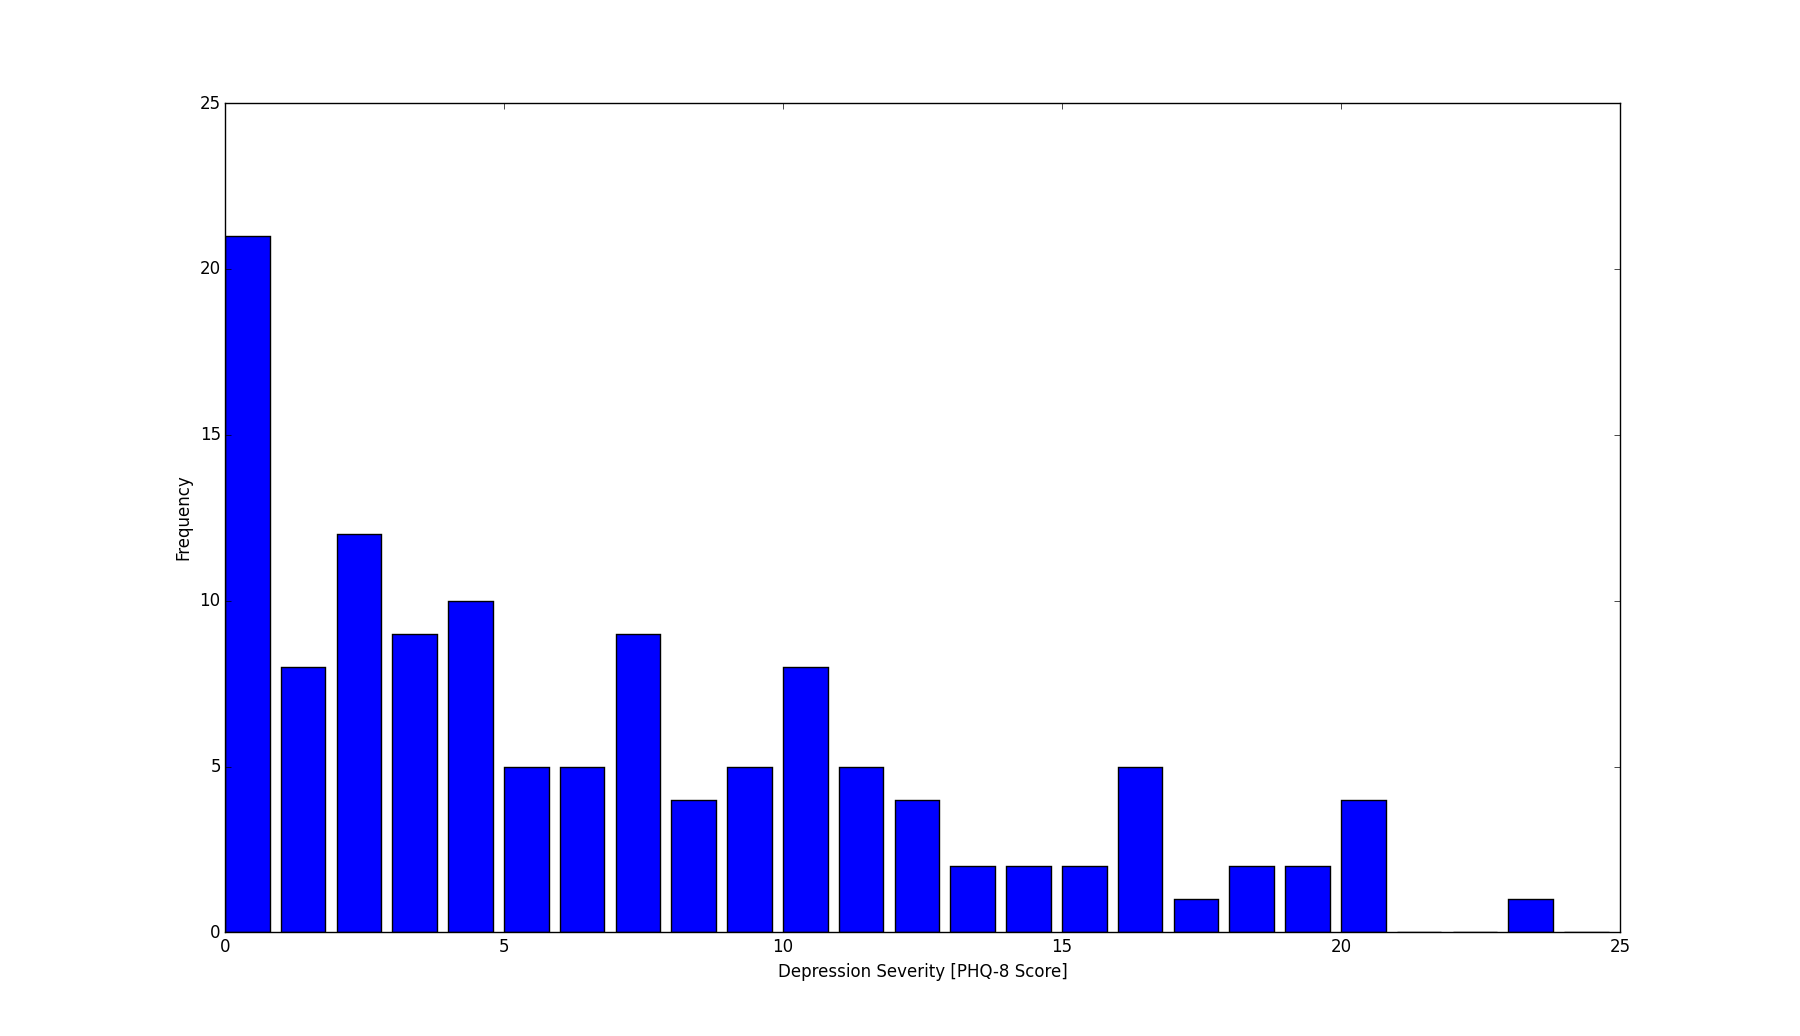
\includegraphics[width=0.5\textwidth]{histogram_phq8}
	\caption{Histogram of the PHQ-8 scores}
	\label{histogram_phq8}
	\end{figure}
	
	The depression data used in AVEC 2016 was obtained from the benchmarking database, Distress Analysis Interview Corpus - Wizard of Oz (DAIC-WOZ). 
	Data collected from DAIC-WOZ include raw audio and video recordings and the corresponsing PHQ-8 score (from 0 to 24) \cite{jad2008}. Hence, we would 
	need to pre-process the auditory data before we use it in our experiment. The pre-processing is briefly discussed in the section below.
	The distribution of the depression severity scores in the dataset is given in Figure \ref{histogram_phq8}. 
	The data provided are split into 2 sets: training and development.
	An overview of the data is given in Table \ref{summary_table}.

 	\begin{table}[h]
 		\begin{center}
  			\begin{tabular}{ | r | c | c | c | }
    			\hline
			 		& \bfseries Training	& \bfseries Development 	& \bfseries All \\ \hline
			 $n$		& 95 			& 31 				& 126 \\ \hline
			 $\mu$	& 6.326 		& 7.548			& 6.626 \\ \hline
			 $\sigma$	& 5.597 		& 6.690 			& 5.909 \\ \hline
			 \end{tabular}
		\end{center}
 	\caption{Summary of Datasets provided}
 	\label{summary_table}
 	\end{table}

	\subsection{Pre-processed data}
	Since the focus of this paper is the prediction of the PHQ-8 score, we will not describe the pre-processing step in detail.
	We used standard signal processing techniques to extract the 4 audio feature sets (Energy, MFCC, Magnitude Spectrum, Zero-crossing) as presented in the Modelling 
	and Approach section.
	Each audio feature set comprises of several individual features and the breakdown of the actual number of feature columns is summarized in Table \ref{no_features}.

 	\begin{table}[h]
 		\begin{center}
  			\begin{tabular}{ | r | c | }
    			\hline
			 \bfseries Audio Feature Sets 	& \bfseries Number of features \\ \hline
			 Magnitude Spectrum		& 512 \\ \hline
			 MFCC 				& 12 \\ \hline
			 Energy 				& 1 \\ \hline
			 Zero-Crossing Rate 		& 1 \\ \hline
			 \bfseries Total			& \bfseries 526 \\ \hline
			 \end{tabular}
		\end{center}
 	\caption{Number of features extracted}
 	\label{no_features}
 	\end{table}

 	\subsection{Measure of Accuracy}
	AVEC 2016 provided a baseline classifier that consistently predicts the PHQ-8 score with $\text{RMSE}=6.7418$ \cite{avec2016}. 
	In order to provide a meaningful and consistent comparison to the baseline provided, we used the same Root Mean Square Deviation Error (RMSE) to measure the 
	error rate on both Training and Development datasets. 
	RMSE (Equation \ref{eq:rmse}) is a commonly used in the machine learning community to measure the differences between the values predicted by a model 
	and the ground truth \cite{Dhanani:EECS-2014-131}. 
	\begin{equation}\label{eq:rmse}
  	\text{RMSE} = \sqrt{\frac{\sum_{t=1}^n (\hat y_t - y_t)^2}{n}}
 	\end{equation} 

	\subsection{Feature Selection}
	Feature selection is the process of selecting a subset of relevant features including variables or predictors to be used in a model for machine learning. 
	The purpose of feature selection is to reduce the complexity of a model to more easily be interpreted. 
	The benefit is three-fold: improving the prediction performance of the predictors, providing faster and most cost-effective predictors, 
	and providing a better understanding of the underlying process that generated the data \cite{Guyon2003}.\\
	
	Since we have more features than data points, it tends to lead to overfitting \cite{Smith2011}. 
	Therefore feature selection is first performed on the data before applying machine learning. 
	The feature selection algorithms used are popular and are taken from scikit-feature, a feature selection library \cite{li2016feature}: CIFE \cite{Lin2006}, Relief 	
	\cite{Rob2003}, CFS \cite{HALLHALL}. 
	We will not go into detail as feature selection is not the main focus of the report.
	
	\subsection{Experimental Setup}
	We compared the proposed GP models against state-of-the-art machine learning models as mentioned in the previous section. 
	For the ease of testing, all implementations of the algorithms except for GP ARD come from the popular machine learning library, Scikit Learn \cite{scikit-learn}. 
	We used the implementation of GP ARD from GPy, a Gaussian Processes framework in Python \cite{gpy2014}.
	The hyper-parameters are either determined by the defaults used in either libraries or some reasonable defaults were used.
	Each machine learning model is trained against the training set and thereafter tested against the development set using RMSE as the error metric. 
	The entire experimental process is shown in Figure \ref{process}. \\
 
 	\begin{comment}
	\begin{table}[h]
  		\begin{center}
   			\begin{tabular}{ | r | c |}
	    		\hline
			Algorithm & Hyper-parameters \\ \hline\hline
			K-Nearest Neighbors        & x \\ \hline
			SVM - Linear               & x \\ \hline
			SVM - RBF                  & x \\ \hline
			Decision Tree              & x \\ \hline
			Random Forest              & x \\ \hline
			AdaBoost                   & x \\ \hline
			Naive Bayes                & x \\ \hline
			GP ARD  	           & x \\ \hline
			GP Isotropic Matern        & x \\ \hline
			GP Dot Product 	           & x \\ \hline
			\end{tabular}
		\end{center}
		\caption{List of Machine Learning Algorithms with their corresponding hyper-parameters}
		\label{list_mls}
	\end{table}
 	\end{comment}
 	
	\begin{figure}[h]
 		\begin{center}
		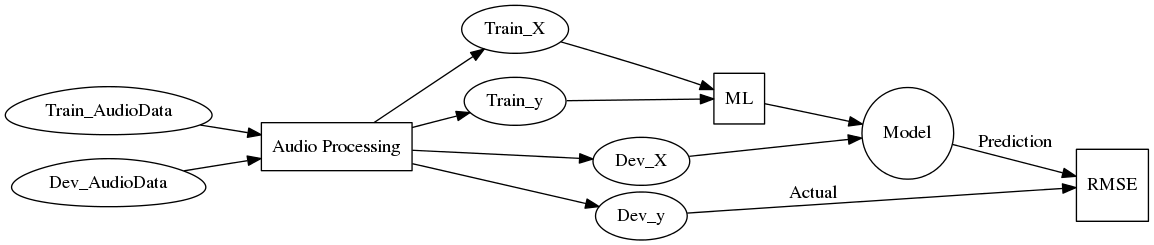
\includegraphics[width=0.48\textwidth]{process} 
  		\end{center}
  		\caption{Experimental process}
  		\label{process} 
 	\end{figure}
 	\begin{comment}
	@startuml
	digraph g {
		graph [rankdir=LR];
	 	ML,RMSE[shape=square];
		Model[shape=circle];
		ap[shape=rect label="Audio Processing"];
		Train_AudioData,Dev_AudioData[shape=egg];
		Train_AudioData -> ap;
		ap -> Train_X;
		ap -> Train_y;
		ap -> Dev_X;
		Dev_AudioData -> ap;
		ap -> Dev_y;
		Train_X -> ML;
		Train_y -> ML;
		ML -> Model
		Dev_X -> Model
		Model -> RMSE[label=Prediction]
		Dev_y -> RMSE[label=Actual]
	}
	@enduml
 	\end{comment}

	\subsection{Results}
	We first ran the experiment across the dataset using all 526 features, without feature selection. 
	As we would expect \cite{Cawley2014}, the results are unacceptable as the ratio of the number of features to the number of data points is too high,
	resulting in possible overfitting. 
	The results of the initial experiment is illustrated in Figure \ref{results_all}. 
	We would expect the GP ARD would be able to theoritcally extract relevant features and improve prediction.
	However, we have observed experimentally that GP ARD performs poorly, along with other GPs. \\

	\begin{figure}[h]
 		\begin{center}
		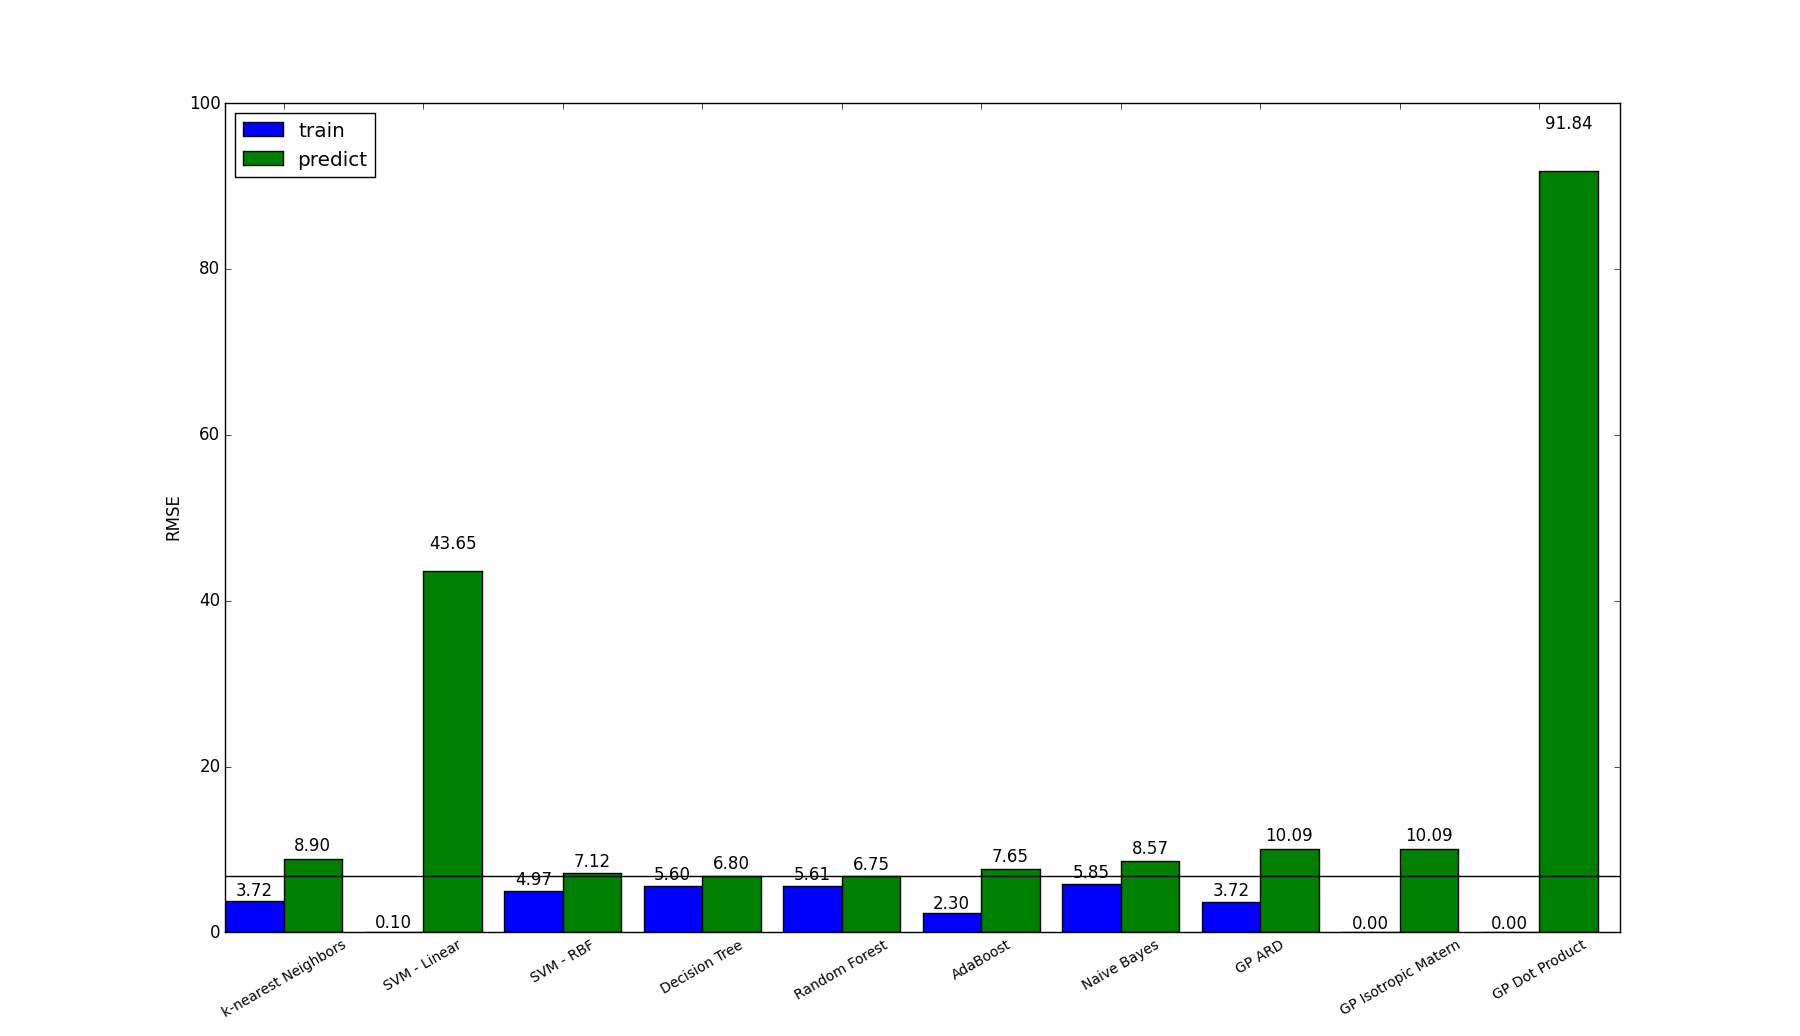
\includegraphics[width=0.5\textwidth]{results_all} 
  		\end{center}
  		\caption{Results across all features}
  		\label{results_all}
 	\end{figure}
	
	We repeated the experiment with feature selection and ran each of the feature subset gathered from the feature selection algorithms against each of the machine 
	learning algorithms. 
	We observed that Relief, CIFE and CFS selected a large number of MFCC features. 
	The number of features in each feature subset is shown in Table \ref{feat_subset}. 
	This confirms our assumption that MFCC gives the best predictive power in PHQ-8 depression severity prediction. 
	Hence, we also ran the experiment using only MFCC features. 
	The best results across all feature subsets are shown in Figure \ref{results_best} and in Table \ref{rmse_results}. The line shown across the 
	bar chart represents the baseline RMSE provided. \\

 	\begin{table}[h]
 		\begin{center}
  			\begin{tabular}{ | r | c | }
    			\hline
			 \bfseries Feature Selection 	&\bfseries Number of features \\ \hline
			 MFCC           			& 12 \\ \hline
			 CIFE        				& 3 \\ \hline
			 Relief 				& 23 \\ \hline
			 CFS 					& 6 \\ \hline
			 All 					& 526 \\ \hline
			 \end{tabular}
		\end{center}
 	\caption{Feature subsets}
 	\label{feat_subset}
 	\end{table}

	\begin{figure}[h]
 		\begin{center}
		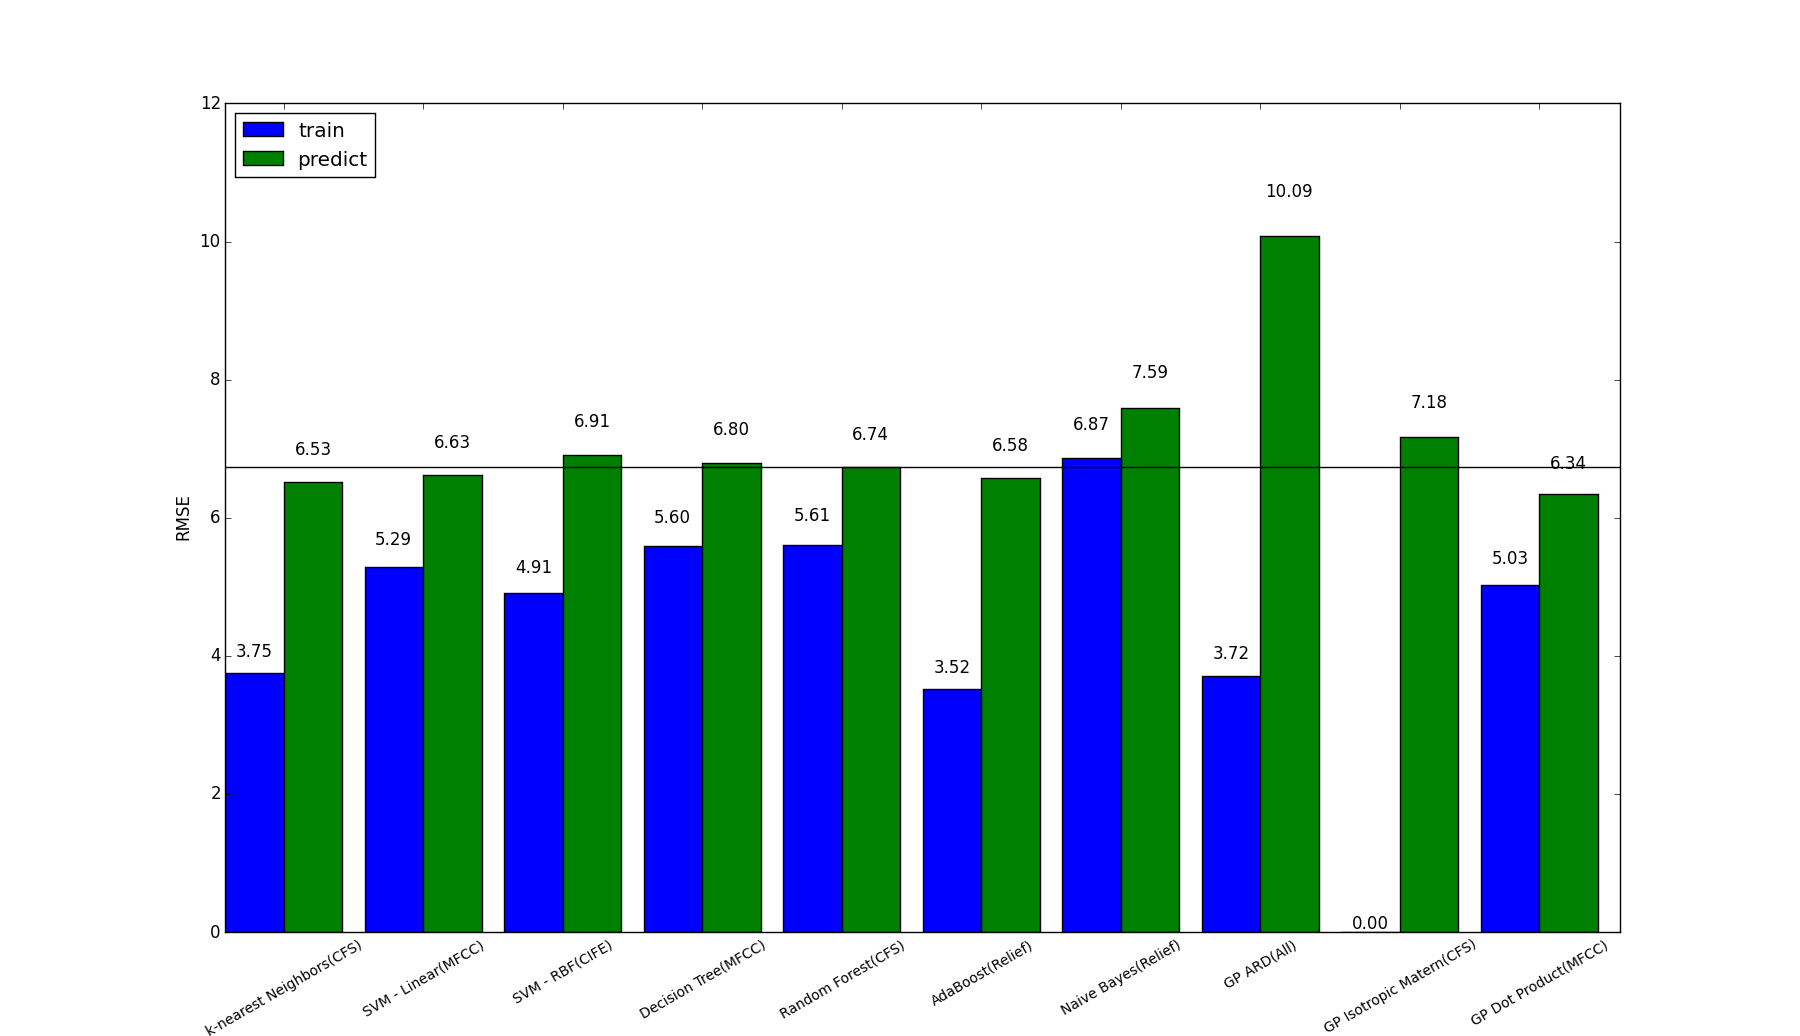
\includegraphics[width=0.5\textwidth]{results_best} 
  		\end{center}
  		\caption{Best Results across all feature subsets}
  		\label{results_best}
 	\end{figure}

	\begin{table}[h!]
		\begin{center}
			\begin{tabular}{ | r | c | c | c | }
			\hline
			\multirow{2}{*}{\bfseries Algorithm}	& \multirow{2}{*}{\bfseries Subset}	& \multicolumn{2}{c|}{\bfseries RMSE} \\\cline{3-4}
									&						& \bfseries Train 	& \bfseries Dev \\ \hline
			\bfseries GP Dot Product  	& \bfseries MFCC  & \bfseries 5.03 & \bfseries 6.34 \\ \hline
			AdaBoost              				& Relief					& 3.55 		& 6.52 \\ \hline
			K-Nearest Neighbors   			& CFS 					& 3.75 		& 6.53 \\ \hline
			SVM - Linear          				& MFCC  					& 5.29 		& 6.63 \\ \hline
			Random Forest         			& CFS   					& 5.61 		& 6.75 \\ \hline
			Decision Tree         				& MFCC  					& 5.60 		& 6.80 \\ \hline
			SVM - RBF             				& CIFE  					& 4.91 		& 6.91 \\ \hline
			GP Isotropic Matern   			& CFS   					& 0.00 		& 7.18 \\ \hline 
			Naive Bayes           				& Relief					& 6.87 		& 7.59 \\ \hline
			GP ARD                				& All   						& 3.72 		& 10.09 \\ \hline

			\end{tabular}
		\end{center}
		\caption{RMSE Results}
		\label{rmse_results}
	\end{table}
	
	As expected, the models perform better with the MFCC feature set. 
	Unexpectedly, the simple GP dot product model, trained with 12 features and 95 data points, outperforms all other machine learning models in our tests. 
	Our results also confirms the initial assumption that MFCC is an appropriate feature set to be used in emotion and therefore depression prediction and that GP is 
	applicable and feasible in predicting PHQ-8 scores.

	\section{Conclusion}	
	Our work has succesfully shown that GP is a good model for this problem and can predict PHQ-8 better than state-of-the-art machine learning models. 
	In addition to being on par or better at prediction, GP can inherently provide an estimate of prediction uncertainty. 
	This allows the user to gauge the model's confidence of the prediction, and to make more informed decisions based on both the prediction and its uncertainty. 
	We can also intelligently supplement more data to our training set based on the prediction uncertaintly. 
	Therefore, after considering both results and GP's advantages, we conclude the GP Dot Product trained using MFCC feature set is a good model for 
	depression prediction.
	
	\section{Further Work}
	For this experiment, we only used machine learning algorithms with their default parameters. 
	An aspect that deserves further exploration is to perform automatic hyper-parameter optimization
	across all the machine learning algorithms to fine-tune each model's performance. 
	In particular, we can try Hyperopt-sklearn \cite{Komer2014HyperoptsklearnAH} or GP based hyper-parameter tuner. 
	We opine that with hyper-parameter tuning, we can predict PHQ-8 scores better and can have a more objective comparison of the different learning algorithms.
	
	\section{Contributions}
	\begin{itemize}
		\item \textbf{Antoine Charles Vincent Garcia}: 
		Scripting the program, setting up machine learning libraries, running tests and generation of the utility function.
		\item \textbf{Chan Jun Wei}: 
		Scripting the program, setting up machine learning libraries, running tests and generation of the utility function.
		\item \textbf{Chen Tze Cheng}: 
		Scripting the program, setting up machine learning libraries, running tests and generation of the utility function.
		\item \textbf{Eric Ewe Yow Choong}: 
		Formatting the report as well as research and writing up of the technical approach section.
		\item \textbf{Han Liang Wee, Eric}: 
		Retrieving data, testing as well as research and writing up of the technical approach section.
		\item \textbf{Ho Wei Li}: 
		Research, vetting of the report and writing up of the motivation and introduction of the experiment. \\
	\end{itemize}
	
	\bibliographystyle{aaai}
	{\scriptsize \bibliography{references}}

\end{document}
